\documentclass[10pt]{article}
\usepackage[utf8]{inputenc}
\usepackage[T1]{fontenc}
\usepackage{amsmath}
\usepackage{amsfonts}
\usepackage{amssymb}
\usepackage[version=4]{mhchem}
\usepackage{stmaryrd}
\usepackage{graphicx}
\usepackage[export]{adjustbox}
\graphicspath{ {./images/} }
\usepackage{caption}
\usepackage{bbold}

\begin{document}
\captionsetup{singlelinecheck=false}
\section*{Two Ions in A Linear Trap}
$\rightarrow$ A PATHWAY TOWRESS ION-QUBIT QUANTUM COMPUTATION (TRAPPED Iow)\\
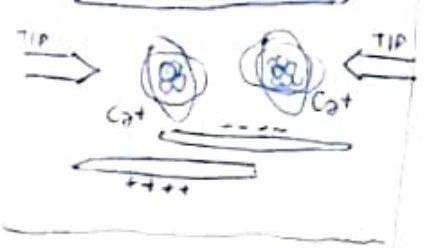
\includegraphics[max width=\textwidth, center]{2025_10_16_f28de32ab20bd0ac9bbfg-1(1)}

\begin{figure}[h]
\begin{center}
  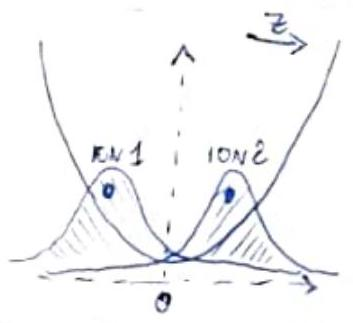
\includegraphics[width=\textwidth]{2025_10_16_f28de32ab20bd0ac9bbfg-1(2)}
\captionsetup{labelformat=empty}
\caption{\textbackslash uparrow\$\\
CIASSICAL EQCILIBRIVH POSITION\\
(EUST A NUMBER, NOT AN OP.)}
\end{center}
\end{figure}

\$\textbackslash hat\{z\}\textit{\{J\} \textbackslash rightarrow \textbackslash hat\{z\}}\{J\}\^{}\{\textbackslash prime\}=\textbackslash hat\{z\}\textit{\{J\}-\textbackslash bar\{z\}}\{J\} \textbackslash hat\{\textbackslash mathbb\{1\}\}

10N MASS\\
$C_{3}^{+} \approx M_{\text {prorov }} \cdot 40$\\
$\underline{x \text { ADY DIMENSIONS } \rightarrow \text { TIGHTLY CONEINED } x=y=0 \text { THUS }}$\\
$H=\frac{\frac{\text { KINETIC }}{p_{1}^{z^{2}}+p_{2}^{z^{2}}}}{2 m}+\frac{\text { TRAP }}{2 m \omega_{1}^{2}\left(z_{1}^{2}+z_{2}^{2}\right)}+\frac{e^{2}}{4 \pi \varepsilon_{0}\left|z_{1}-z_{2}\right|}$\\
Fno analytical exact solution:\\
I CAN DO SMALL-OSCIUATION EXAANSION (AND CHECK "A POSTERIORI" CONSISTENCY)\\
COMMUTATORS ARE THE SAME\\
$\left[z_{i}^{\prime}, p_{J}\right]=\left[z_{i}, p_{J}\right]-z_{i}\left[1, p_{J}\right]$\\
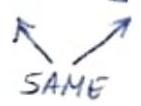
\includegraphics[max width=\textwidth, center]{2025_10_16_f28de32ab20bd0ac9bbfg-1}

LEIND $\left.\bar{z}_{3}\right\rangle$ FIRST OF AU, $\stackrel{2}{0}_{\text {LEFT }}^{2} \longrightarrow$ SO $\bar{z}_{1}>\bar{z}_{2}$ THUS $\frac{1}{\left|\bar{z}_{1}-\bar{z}_{2}\right|}=\frac{1}{\bar{z}_{1}-\bar{z}_{2}} \begin{aligned} & \text { CLASSICAL } \\ & \text { EQUICIBRICM: }\end{aligned} \quad \dot{p}=0\binom{\text { NO }}{\text { ACLELER. }} \quad 0=-p=+\left.\frac{\partial H}{\partial q} \leadsto \frac{\partial H}{\partial \vec{z}_{y}}\right|_{\bar{z}_{y}} 0$

$$
\begin{aligned}
& \left.\frac{\partial H}{\partial z_{1}}\right|_{\bar{z}_{1}, \bar{z}_{2}}\left\{\begin{array} { l } 
{ m \omega _ { T } ^ { 2 } \overline { z } _ { 1 } - \frac { e ^ { 2 } } { 4 \pi \varepsilon _ { 0 } } \frac { 1 } { ( \overline { z } _ { 1 } - \overline { z } _ { 2 } ) ^ { 2 } } = 0 } \\
{ \frac { \partial H } { \partial z _ { 2 } } | _ { \overline { z } _ { 1 } , \overline { z } _ { 1 } } }
\end{array} \left\{\begin{array}{l}
m \omega_{T}^{2} \bar{z}_{2}+\frac{e^{2}}{4 \pi \varepsilon_{0}} \frac{1}{\left(\bar{z}_{1}-\bar{z}_{2}\right)^{2}}=0
\end{array}\right.\right.
\end{aligned}
$$

SUHMING THE\\
EQUATIONS $\bar{z}_{2}=-\bar{z}_{1}$ SUBSTITUTE

$$
m \omega_{T}^{2} \bar{z}_{1}-\frac{e^{2}}{16 \pi \varepsilon_{0}} \frac{1}{\bar{z}_{1}^{2}}=0
$$

EQUILIBRIOM ANS NOW\\
$\hat{z}_{j}=\bar{z}_{j} \mathbb{1}+\hat{z}_{j}^{\prime}$ SO

$$
\hat{z}_{2}^{2}=\bar{z}_{2}^{2} \hat{\mathbb{1}}+2 \bar{z}_{1} \hat{z}_{2}^{\prime}+\hat{z}_{2}^{\prime 2}{ }^{\text {EXACT }}
$$

$$
\left|\hat{z}_{1}-\hat{z}_{2}\right|^{-1} \approx\left(\hat{z}_{1}-\hat{z}_{2}\right)^{-1}=\frac{\hat{1}}{\left(\bar{z}_{1}-\bar{z}_{2}\right)}-\frac{\left(\hat{z}_{1}^{\prime}-\hat{z}_{2}^{\prime}\right)}{\left(\bar{z}_{1}-\bar{z}_{2}\right)^{2}}+\frac{\neq A}{\mathbb{A}} \frac{\left(\hat{z}_{1}-\hat{z}_{2}^{\prime}\right)^{2}}{\left(\bar{z}_{1}-\bar{z}_{2}\right)^{3}}+O\left(\hat{z}_{j}^{3}\right)
$$

$$
\begin{aligned}
H_{\text {SMOL }}=\frac{p_{1}^{2^{2}}+p_{2}^{2^{2}}}{2 m} & +\frac{m \omega_{1}^{2}}{2}\left(\frac{\bar{z}_{1}^{2} / 1}{1}+\bar{z}_{2}^{2} / 11+2 \bar{z}_{1} \hat{z}_{1}^{\prime}+2 \bar{z}_{2} \hat{z}_{2}^{\prime}+\hat{z}_{1}^{\prime 2}+\hat{z}_{2}^{\prime 2}\right)+ \\
& \frac{e^{2}}{4 \pi \varepsilon_{0}}\left(+\frac{11}{\bar{z} / \bar{z} / \overline{z_{2}}}-\frac{\hat{z}_{1}^{\prime}-\hat{z}_{2}^{\prime}}{\left(\bar{z}_{1}-\bar{z}_{2}\right)^{2}}+\frac{\left(\hat{z}_{1}^{\prime}-\hat{z}_{2}^{\prime}\right)^{2}}{\left(\bar{z}_{1}-\bar{z}_{2}\right)^{3}}\right)+\theta\left(\hat{z}_{3}^{\prime 3}\right) \quad \begin{array}{c}
\text { SHITY AWAY } \\
\text { THE } \\
\text { CONTANTS }
\end{array}
\end{aligned}
$$

$$
\left.\begin{array}{c}
\text { ISOLATING } \\
\text { FIRST-ORSER } \\
\text { TERMS } \hat{z}_{1}^{\prime}
\end{array} I^{0} \Delta\right\rangle \hat{z}_{1}^{\prime}(\underbrace{m \omega_{r}^{2} \bar{z}_{1}-\frac{e^{2}}{4 \pi \varepsilon_{0}\left(\bar{z}_{1}-\bar{z}_{2}\right)^{2}}}_{=0})+\hat{z}_{2}^{\prime}(\underbrace{m \omega_{r}^{2} \bar{z}_{2}+\frac{e^{2}}{4 \pi \varepsilon_{0}\left(\bar{z}_{1}-\bar{z}_{2}\right)^{2}}}_{\text {BY CONSTRUCTION }})
$$

ISOLATING\\
$\underset{\substack{\text { SECCND-RRDER } \\ \text { TERMS }}}{\text { ISOLATING }}$ II $^{\sigma} \Delta>\frac{m \omega_{T}^{2}}{2}\left(\hat{z}_{i}^{2}+\hat{z}_{i}^{2}\right)+\left(\hat{z}_{i}-\hat{z}_{i}^{\prime}\right)^{2} \frac{e^{2}}{4 \pi \varepsilon_{0}}\left(\bar{z}_{1}-\bar{z}_{2}\right)^{-3}$

$$
\frac{e^{2}}{4 \pi \varepsilon_{0}}\left(\bar{z}_{1}-\bar{z}_{2}\right)^{-3}=\frac{e^{2}}{4 \pi \varepsilon_{0}} \frac{1}{\left(2 \bar{z}_{1}\right)^{3}}=\frac{e^{2}}{32 \pi \varepsilon_{0}}\left(\frac{16 \pi \varepsilon_{0} \pi \omega_{T}}{e^{2}}\right)=\frac{1}{2} m \omega_{T} \quad \forall
$$

$\begin{aligned} \text { H SAMR }_{\text {OSCIUATIONS }} & =\frac{1}{2 m}\left(p_{1}^{2}+p_{2}^{2}\right)+\frac{m \omega_{1}^{2}}{2}\left(z_{1}^{2}+z_{2}^{2}+\left(z_{1}^{\prime}-z_{2}^{\prime}\right)^{2}\right)+ \\ { }^{\tau} \text { COUPLED HARMONIC OSCILATORS (YEAM, NO BIG SURARISE) } & \end{aligned}$\\
center-of-mass \& relative\\
COORINATE

HOLENICH $P=p_{1}^{z}+p_{12}^{z}$

$$
z=z_{1}^{\prime}-z_{2}^{\prime}
$$

$$
p=\frac{p_{1}^{t}-p_{2}^{2}}{2}
$$

WHEH MEANS

$$
\begin{aligned}
& p_{1}^{z}=\frac{p}{2}+p \quad p_{2}^{z}=\frac{p}{2}-p \quad z_{1}^{\prime}=z+\frac{z}{2} \quad z_{2}^{\prime}=z-\frac{z^{0}}{2} \quad \text { AND THUS } \\
& \left(p_{1}^{z^{2}}+p_{2}^{z^{2}}\right)=\frac{p^{2}}{2}+2 p^{2} \quad\left\|\left(z_{1}^{2}+z_{2}^{2}\right)=2 z_{1}^{2}+\frac{z^{2}}{2}\right\|\left(z_{1}^{1}-z_{2}^{1}\right)^{2}=z^{2}
\end{aligned}
$$

$$
H_{\text {SHAM }}=\left[\frac{p^{2}}{4 m}+m \omega_{T}^{2} z^{2}\right]+\left[\frac{p^{2}}{m}+\frac{m \omega_{T}^{2}}{2}\left(\frac{z^{2}}{2}+z^{2}\right)\right]+\theta\left(z_{T}^{3}\right)
$$

CENTER-OF-HASS HARMONIC OSCILLATOR\\
(recative) "stretch mose" HARMONIC OSCIWATOR

DECOUPED PROBLEMS

COM\\
HODE

$$
Z=\sqrt{\frac{\hbar}{4 m \omega_{T}}}\left(a_{\mathrm{COH}}+a_{\mathrm{COH}}^{+}\right)+P=i \sqrt{\hbar m \omega_{T}}\left(a_{\mathrm{COH}}^{+}-a_{\mathrm{COH}}\right)
$$

$$
\underset{0 \rightarrow 0}{\leftarrow}
$$

\begin{center}
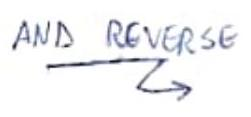
\includegraphics[max width=\textwidth]{2025_10_16_f28de32ab20bd0ac9bbfg-3}
\end{center}

$$
a_{c+1}=\sqrt{\frac{m \omega_{T}}{\hbar}} Z+i \sqrt{\frac{1}{4 \hbar m \omega_{T}}} P \quad\left[a_{1}, a_{1}^{+}\right]=1
$$

\section*{STRETCH MODE}
$$
z=\sqrt{\frac{\hbar}{\sqrt{3} m \omega_{T}}}\left(a_{S}+a_{S}^{+}\right) ; p=i \sqrt{\frac{\sqrt{3} \hbar m \omega_{T}}{4}}\left(a_{S}^{+}-a_{S}\right)
$$

$$
\leadsto a_{5}=\sqrt{\frac{\sqrt{3} m \omega_{T}}{4 \hbar}} z+i \sqrt{\frac{1}{\sqrt{3} \hbar m \omega_{T}}} p
$$

$$
H_{\substack{\text { SHALL } \\ \text { OSC. }}}=\hbar \omega_{T}\left(a_{\text {GOH }}^{+} a_{\text {COM }}+\frac{1}{2}\right)+\hbar \sqrt{3} \omega_{T}\left(a_{S}^{+} a_{S}+\frac{1}{2}\right)+\phi_{C O N T}(\ldots)
$$

$\left\{\begin{array}{l}\text { THE STRETCH MODE IS } \sqrt{3} \approx 1.73 \text { TIMES FASTER THAN THE COM MODE, } \\ \text { THAT IS, SEVERAL MHZ AWAY- Back TO lab coordinates }\end{array}\right.$

$$
\begin{aligned}
& z_{1,2}= \pm \bar{z}_{1}+z_{12}^{\prime}= \pm \bar{z}_{1}+z \pm \frac{z}{2} \\
& z_{1,2}= \pm \bar{z}_{1}+\sqrt{\frac{\hbar}{4 m \omega_{T}}}\left(a_{G H}+a_{G M}^{+} M\right) \pm \sqrt{\frac{\hbar}{4 m \sqrt{3} \omega_{T}}}\left(a_{S}+a_{S}^{+}\right)
\end{aligned}
$$

Adding a FOCUSED Laser, SAY, ON ION. 1\\
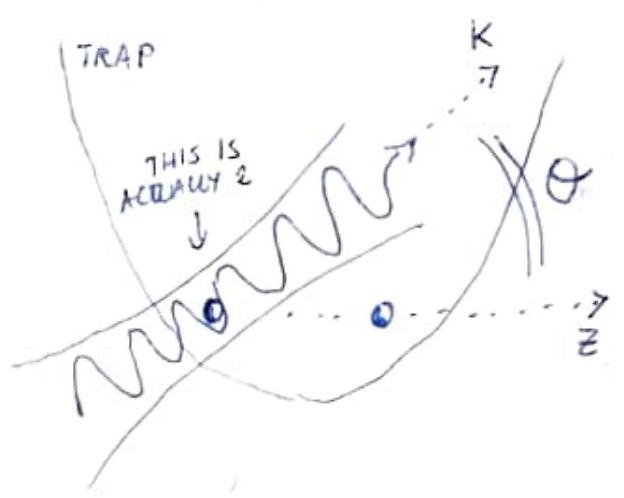
\includegraphics[max width=\textwidth, center]{2025_10_16_f28de32ab20bd0ac9bbfg-3(1)}

LIENT-ATOM COUPING (DIPOLE)

$$
\begin{aligned}
H_{\text {WEING }}=-\vec{d} \cdot \vec{E}(\vec{r})=\ldots= & \frac{10 N 1}{\downarrow} \\
= & -\hbar \Omega_{\text {HAB }} \mid e x g_{1} \cos \left(c k t-\cos \theta k z_{1}\right)+\text { h.c. } \\
& c k=\omega_{L}
\end{aligned}
$$

$$
=-\hbar \Omega \left\lvert\, e x g_{1} \cos (c k t-\underbrace{\cos \theta k \bar{z}_{1}}_{\phi_{0}}-\underbrace{\cos \theta k \sqrt{\frac{\hbar}{4 m \omega_{r}}}}_{\eta_{C O H}}\left(a_{C O H}+a_{C O H}^{+}\right)-\underbrace{\cos \theta k \sqrt{\frac{\hbar}{4 \sqrt{3} m \omega_{r}}}}_{\eta_{S}}\left(a_{S}+a_{S}^{+}\right))\right.
$$

$$
\begin{aligned}
& H_{\text {FULL }}^{(L A B)}=\hbar \omega_{\text {eg }}^{\sum \sum \text { lexel }}+\hbar \omega_{T} a_{\text {COM }}^{+} a_{C O M}+\sqrt{3} \hbar \omega a_{S}^{+} a_{S}+H_{\substack{\text { ABTOH } \\
\text { IVIT. } \\
\text { IVI }}} \\
& \underset{\text { FRAME }}{\operatorname{ROTATINE}} U(t)=e^{-i \omega_{L} t \sum_{j} \mid e x e t_{j}+i \psi_{0}} \quad \stackrel{(g N D)}{R W A} \quad\left|\omega_{e g}-\omega_{l}\right|, \Omega \ll \omega_{e g}, \omega_{l} \\
& -\Delta \\
& H_{\text {RWA }}^{\text {(ROTC) }}=\hbar(\overbrace{\omega_{\text {eg }}-\omega_{L}}) \sum_{\text {S }}|e \times e|_{S}+\hbar \omega_{T} a_{C_{O M}}^{+} a_{C_{O M}}+\sqrt{3} \hbar \omega_{T} a_{S}^{+} a_{S}+ \\
& \left\{-\frac{\hbar \Omega}{2}|e x g|_{1} e^{-i \eta_{C O M}\left(a_{C O M}+a_{C O M}^{+}\right)} e^{-i \eta_{S}\left(a_{S}+a_{S}^{+}\right)}+\right.\text {h.c. } \\
& -\frac{\hbar \Omega}{2} \operatorname{lexg} 1_{1}\left(1-i \eta_{C_{O H}}\left(a_{C_{O M}}+a_{C_{O M}}^{+}\right)-i \eta_{s}\left(a_{s}+a_{s}^{+}\right)+\theta\left(\eta^{2}\right)\right)+\text { h.c. }
\end{aligned}
$$

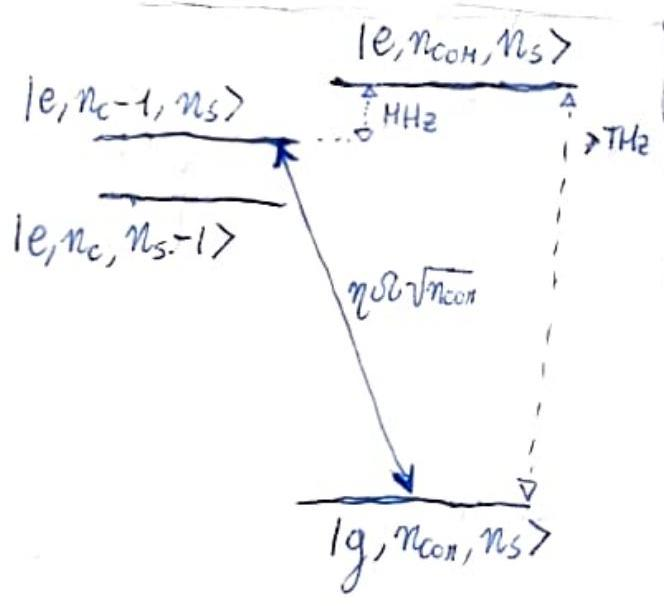
\includegraphics[max width=\textwidth, center]{2025_10_16_f28de32ab20bd0ac9bbfg-4}\\
$\leftarrow$ ENERGY SELECTION:\\
I don specifically address (for example) "The red sinebans of the com mode"

NAMELY

$$
\begin{gathered}
\left|\Delta+\omega_{T}\right| \approx K H Z \ll \omega_{T} \approx \mathrm{MHZ} \\
\text { BUT THEN }
\end{gathered}
$$

$$
\begin{aligned}
& \underbrace{\Delta \approx-\omega_{r}}_{K H_{z}} \\
& \downarrow \\
& H_{\text {jual }}=\hbar\left(\omega_{T}+\varepsilon\right)|e x e|_{1}+\hbar \omega_{T} a_{C O M}^{+} a_{C O M}+ \\
& +\frac{\hbar \eta \Omega}{2}\left(i \sigma_{1}^{+} a_{G M}^{-} i \sigma_{1}^{-} a_{G M}^{+}\right)+\text {iecouples stuff. } \\
& \uparrow \text { center-of-mass (axial) phonon jaynes cummings } \uparrow
\end{aligned}
$$

\section*{\begin{center}
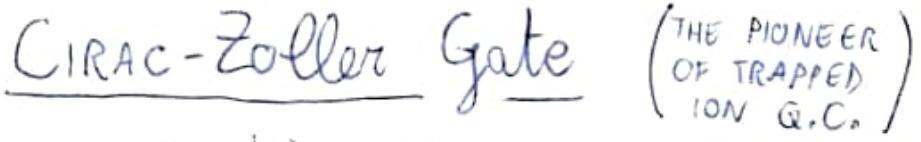
\includegraphics[max width=\textwidth]{2025_10_16_f28de32ab20bd0ac9bbfg-5}
\end{center}}
Ingredients:

2x 3-level Ions (ex. (at)\\
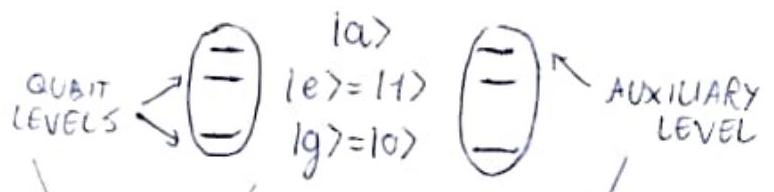
\includegraphics[max width=\textwidth, center]{2025_10_16_f28de32ab20bd0ac9bbfg-5(1)}

2x Forused Lasers\\
1x. Harmonic Ion trap\\
$\rightarrow$ very cols\\
DIFFICULT REQUREMENT:\\
CoM Phonons @ T=O b

\section*{PRELIMINARY}
lasers will be perfectly resonant to a transition, when this happens I can go to an interaction picture\\
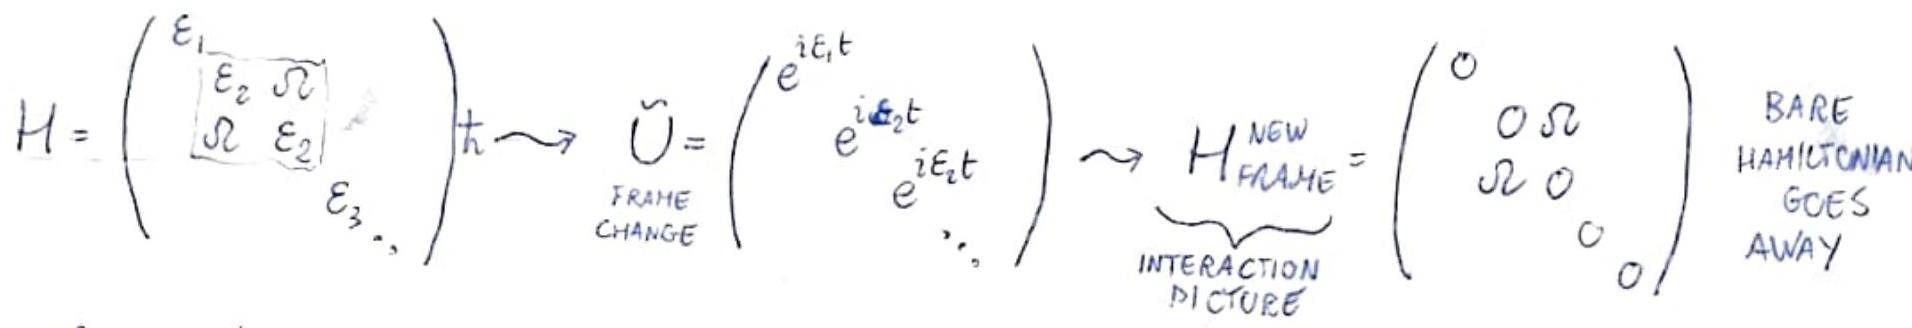
\includegraphics[max width=\textwidth, center]{2025_10_16_f28de32ab20bd0ac9bbfg-5(2)}\\
Laser 1\\
TUNEATO:\\
$|g\rangle_{1} \leftrightarrow|e\rangle_{1}$ RED\\
$\triangle I D E B A N D$

$$
H_{\text {USER-1 }}=\frac{\hbar \eta_{\text {COM }} \Omega_{1}}{2}\left(i \text { lexg }\left.\right|_{1} a_{\text {COM }}+\text { h.c. }\right) \omega_{2} \cong \omega_{\text {eg }}-\omega_{r}
$$

Laver 2\\
TUNED TO:\\
$\begin{aligned} & \text { TONED TO: } \\ & \left.|g\rangle_{2} \leftrightarrow i a\right\rangle_{2} \text { RED } \\ & \text { SIDEBAND }\end{aligned} \quad H_{L 2}=\frac{\hbar \eta_{C O M} \Omega_{2}}{2}\left(i \mid a \times g_{2} a_{C O M}+h . c,\right) \quad \omega_{L} \cong \omega_{a g}-\omega_{T}$\\
STEP 1) Turn on Laser-1 for a time $T_{1}=\frac{\pi}{\eta \Omega_{1}}$ (a $\pi$-pulse)\\
$U_{1}=\exp \left(\frac{\pi}{\eta \Omega_{1}}(-i) \frac{1}{\hbar} H_{1}\right)=\exp \left(-i \frac{\pi}{2}\left(i|\operatorname{exg}| \phi a_{\text {con }}-i \lg \times\left.\right|_{1} a_{\text {corr }}^{+}\right)\right)$\\
This is basically a $\sigma^{\gamma}$ on the states $|g, 1\rangle ;|e, 0\rangle$\\
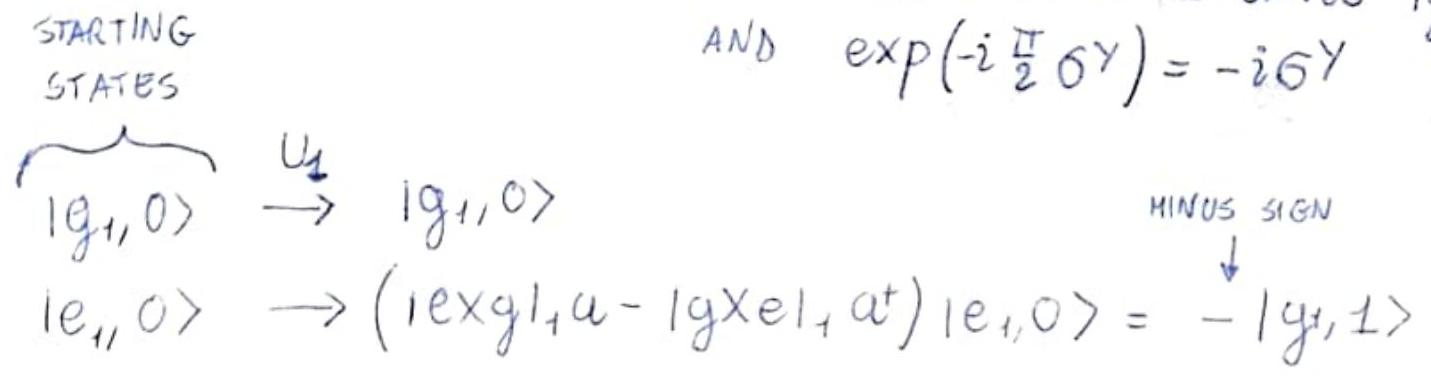
\includegraphics[max width=\textwidth, center]{2025_10_16_f28de32ab20bd0ac9bbfg-5(3)}

$$
e^{i \alpha \sigma}=\cos \alpha \cdot 11+i \sin \alpha \sigma
$$

STED 21 Turn Laser-2 for a time $T_{2}=\frac{2 \pi}{\eta_{\text {con }} \Omega_{2}}$ (a $2 \pi$ pulse)\\
$U_{2}=\exp \left(-\frac{i}{\hbar} \frac{2 \pi}{\eta_{c c H} \Omega_{i}} H_{2}\right)=\exp \left(-i \pi\left(i \mid a \times g l_{2} a_{c O H}+\right.\right.$ h.c. $\left.)\right)$\\
$\overbrace{|g 2,0\rangle}^{\substack{\text { POSSIBLE STARTING } \\ \text { STATES }}} \xrightarrow{U_{2}}|g, 0\rangle$\\
$\left|e_{2}, h\right\rangle \xrightarrow{U_{2}}\left|e_{2}, n\right\rangle$\\
$\left|g_{2}, 1\right\rangle \longrightarrow-\left|g_{1}, 1\right\rangle$\\
Step 3 identical to step 1\\
$U_{3}=U_{1}$ AND $\quad U_{3}\left|g_{1}, 1\right\rangle=+\left|e_{1}, 0\right\rangle$\\
Table of CANONICAL states

\begin{center}
\begin{tabular}{llllll}
\begin{tabular}{l}
$\left|g_{1} g_{2} 0\right\rangle$ \\
$\left|g_{1} e_{2} 0\right\rangle$ \\
$\left|e_{1} g_{2} 0\right\rangle$ \\
$\left|e_{1} e_{2} 0\right\rangle$ \\
\end{tabular} & \begin{tabular}{l}
$\left|g_{1} g_{2} 0\right\rangle$ \\
$\left|g_{1} e_{2} 0\right\rangle$ \\
\end{tabular} & $\longrightarrow$ & \begin{tabular}{l}
$\left|g_{1} g_{2} 0\right\rangle$ \\
$-\left|g_{1} g_{2} 1\right\rangle$ \\
$-\left|g_{1} e_{2} 1\right\rangle$ \\
\end{tabular} & $\xrightarrow{U_{2}}$ & $\left|g_{1} g_{2} 0\right\rangle$ \\
 & - & $\left|g_{1} g_{2} 1\right\rangle$ & \begin{tabular}{l}
$U_{1}$ \\
$-\left|g_{1} g_{2} 0\right\rangle$ \\
$\left|g_{1} e_{2} 0\right\rangle$ \\
\end{tabular} &  & $\left|e_{1} g_{2} 0\right\rangle$ \\
 & $-\left|e_{1} e_{2} 0\right\rangle$ &  &  &  &  \\
\end{tabular}
\end{center}

$\left.\begin{array}{l}\text { AS A } \\ \text { MATRIX }\end{array}\right\} \quad G=U_{1} U_{2} U_{1}=\left(\begin{array}{llll}1 & & & \\ & 1 & & \\ & & 1 & \\ & & -1\end{array}\right) \leftarrow \begin{aligned} & \text { CONTROL } \\ & \text { PHASE-FUP } \\ & \text { GATE }\end{aligned}$\\
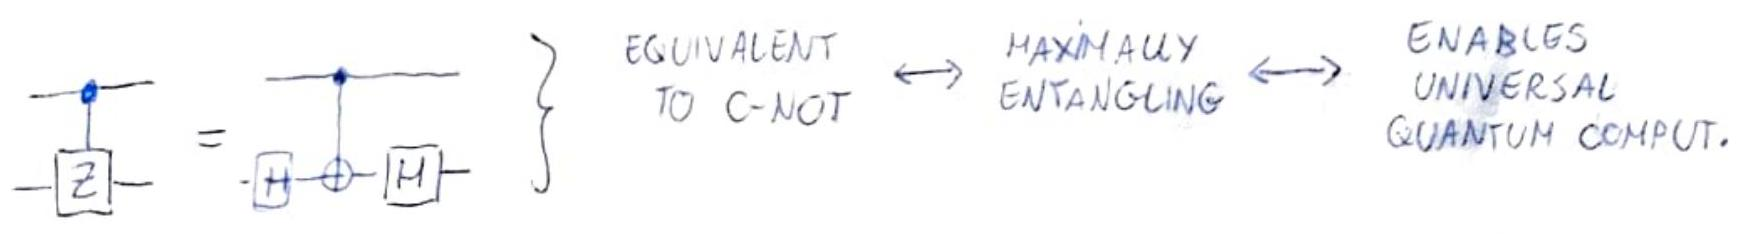
\includegraphics[max width=\textwidth, center]{2025_10_16_f28de32ab20bd0ac9bbfg-6}

OM EASY TO GENERALIZE TO N IONS [PRL 74, 4091(1995)]\\
$\left\{\begin{array}{l}\text { Big } \\ \text { Problem }\end{array} \leadsto \begin{array}{l}\text { T=0 zero temperature phonon } \\ \text { is microkelvin nonsense }\end{array}\right\} \begin{aligned} & \text { Solution: } \\ & \text { Mol Her-S } \text { drensen }(\text { gg })\end{aligned}$


\end{document}